\chapter{Algorithme CRUSH}
\label{crush-algo}

\begin{figure}
  \centering
  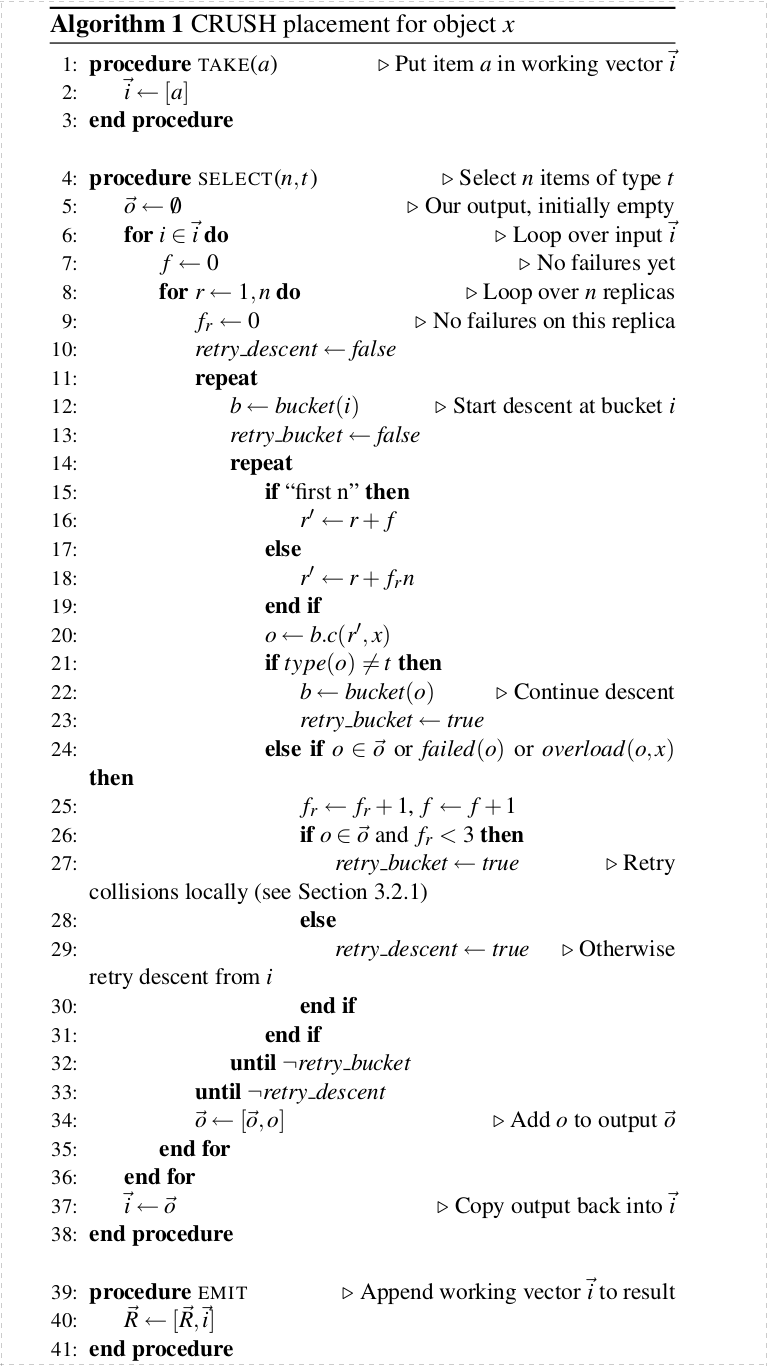
\includegraphics[scale=.5]{./images/algo_crush.png}
  \caption{Détail de l'algorithme CRUSH.}
  \label{chap3:CRUSH_algo}
\end{figure}

\chapter{Mise à jour du noyau  - Debian 8}\label{annexe_noyau_install}

La distribution Debian 8 (Jessie) intègre par défaut une version 3.X du noyau. Dans le cadre de notre installation, nous avons choisi d'utiliser btrfs comme système de fichiers des partitions de stockage Ceph des OSDs, or ce système de fichier est stable depuis les versions 4.X du noyau.

Les commande suivantes permettent de mettre à jour le noyau vers la version stable la plus récente, dans notre cas la 4.9 :
\lstset{emph={echo, sudo,apt,get}}
\vspace{3mm}
\begin{lstlisting}[language=bash] 
  $ sudo echo deb http://http.debian.net/debian jessie-backports main > /etc/apt/sources.list.d/jessie-backports.list
  $ sudo apt-get update
  $ sudo apt-get -t jessie-backports install linux-image-amd64
  $ sudo apt-get -t jessie-backports install linux-headers-amd64
\end{lstlisting}